\documentclass{article}
\usepackage{graphicx}
\usepackage{xcolor}
\usepackage{listings}
\usepackage{hyperref}
\definecolor{vgreen}{RGB}{104,180,104}
\definecolor{vblue}{RGB}{49,49,255}
\definecolor{vorange}{RGB}{255,143,102}

\lstdefinestyle{verilog-style}
{
    language=Verilog,
    basicstyle=\small\ttfamily,
    keywordstyle=\color{vblue},
    identifierstyle=\color{black},
    commentstyle=\color{vgreen},
    numbers=left,
    numberstyle=\tiny\color{black},
    numbersep=10pt,
    tabsize=8,
    literate=*{:}{:}1
}

\begin{document}

\title{ LUT optimization of Fast Fourier Transform }
\author{ Mohankumar Ramachandran }

\maketitle

\begin{abstract}
Fast Fourier Transform (FFT) remains of a great importance due to its substantial role in the field of signal processing and imagery. In this report, multiple designs of 8 point FFT  algorithm is proposed. The developed architecture was implemented using an FPGA . Though, the material resources of the FPGA are limited, particularly the integrated DSP blocks, different approaches are used during the Verilog description with the aim to reduce the necessary number of LUTs. The experimental validation was done using ISIM simulation tool, where the numerical synthesis and the post and route described in Verilog was realized using ISE Design Suite 14.7. The FFT modules of all the implementations were tested using a python script with various corner input test vectors.
\end{abstract}


\section{Cooley–Tukey algorithm }
\label{raw_Cooley_Tukey_algorithm}

\subsection{Overview}
Cooley–Tukey algorithm re-expresses the discrete Fourier transform (DFT) of an arbitrary composite size N = $N_1N_2$ in terms of $N_1$ smaller DFTs of sizes $N_2$, recursively, to reduce the computation time to \textbf{O}(N log N) for highly composite N.

\subsection{Calculation}
This is a direct implementation of Cooley-Turkey Algorithm without any modifications , and for a 8 point FFT , it involves 2 multiplications for a single output calculation. The equations involving the calculation of FFT in shown below. 
$\\\\
t_1=D(0) + D(4);  m_3=D(0) - D(4); \\
t_2=D(6) + D(2);  m_6=j*(D(6)-D(2)); \\
t_3=D(1) + D(5);  t_4=D(1) - D(5); \\
t_5=D(3) + D(7);  t_6=D(3) - D(7); \\ 
t_8=t_5 + t_3;  m_5=j*(t_5-t_3); \\
t_7=t_1 + t_2;  m_2=t_1 - t_2; \\
m_0=t_7 + t_8;  m_1=t_7 - t_8; \\
m_4=sin(\pi/4)*(t_4 - t_6);  m_7=-j* sin(\pi/4)*(t_4 + t_6); \\
s_1=m_3 + m_4;  s2=m_3 - m_4; \\
s_3=m_6 + m_7;  s4=m_6 - m_7; \\
DO(0)=m_0;  DO(4)=m_1; \\ 
DO(1)=s_1 + s_3;  DO(7)=s_1 - s_3; \\
DO(2)=m_2 + m_5;  DO(6)=m_2 - m_5; \\
DO(5)=s_2 + s_4;  DO(3)=s_2 - s_4; \\\\
$
where D and DO are input and output arrays of the complex data $t_1$,…,$t_8$, $m_1$,…,
$m_7$, $s_1$,…,$s_4$ are the intermediate complex results. As we see the algorithm contains only 2 multiplications to the untrivial coefficient sin($\pi$/4) = 0.7071, and 22 real additions and subtractions. The multiplication to a coefficient j means the negation the imaginary part and swapping real and imaginary parts.

\subsection{Implementation}

The below code implements the \hyperref[raw_Cooley_Tukey_algorithm]{Cooley–Tukey algorithm }. inp1,...inp8 are the 16 bit signed floating point inputs of Q format and out1-real , out1-imag, ...,out8-real,out8-imag are the real and imaginary outputs in 16 bit Q format of the FFT8 module.clk , rst are the clock , reset inputs respectively , and output-stb is the output strobe , which is enabled once the output is calculated.


\begin{lstlisting}[style={verilog-style}]
`timescale 1ns / 1ps

module fft8(
	input signed [15:0] inp1,
	input signed [15:0] inp2,
	input signed [15:0] inp3,
	input signed [15:0] inp4,
	input signed [15:0] inp5,
	input signed [15:0] inp6,
	input signed [15:0] inp7,
	input signed [15:0] inp8,
	input clk,
	input rst,
	output signed [15:0] out1_real,
	output signed [15:0] out1_imag,
	output signed [15:0] out2_real,
	output signed [15:0] out2_imag,
	output signed [15:0] out3_real,
	output signed [15:0] out3_imag,
	output signed [15:0] out4_real,
	output signed [15:0] out4_imag,
	output signed [15:0] out5_real,
	output signed [15:0] out5_imag,
	output signed [15:0] out6_real,
	output signed [15:0] out6_imag,
	output signed [15:0] out7_real,
	output signed [15:0] out7_imag,
	output signed [15:0] out8_real,
	output signed [15:0] out8_imag,
	output out_stb
);
	
	localparam signed sin_45 = 16'b00000000_10110101;
	localparam signed sin_315 = 16'b11111111_01001011;

	reg signed [31:0] t1_46,t2_46; 
	reg signed [15:0] t1,t2,t3,t4,t5,t6,t7,t8,m0,m1,m2,m3,m4;
	reg signed [15:0] m7_imag,s1,s2,s3_imag,s4_imag,m5_imag,m6_imag;
	reg output_stb;
	
	initial 
		begin
			output_stb = 1'b0;
		end

	always @( posedge clk )
		begin
			if (rst == 1'b1)
				begin
					output_stb = 1'b0;
				end
			else
				begin
					t1 = inp1 + inp5;
					t2 = inp7 + inp3;
					t3 = inp2 + inp6;
					t5 = inp4 + inp8;
					m3 = inp1 - inp5;
					m6_imag = inp7 - inp3;
					t4 = inp2 - inp6;
					t6 = inp4 - inp8;
					t8 = t5 + t3;
					t7 = t1 + t2;
					m0 = t7 + t8;
					t1_46 = sin_45 * ( t4 - t6);
					m4 = t1_46 [23:8]; 
					m5_imag = t5 - t3;
					m2 = t1 - t2;
					m1 = t7 - t8;
					t2_46 = sin_315 * ( t4 + t6); 
					m7_imag = t2_46 [23:8];
					s1 = m3 + m4;
					s2 = m3 - m4;
					s3_imag = m6_imag + m7_imag;
					s4_imag = m6_imag - m7_imag;
					output_stb = 1'b1;
				end
		end
	assign out1_real = m0;
	assign out1_imag = 16'b0000000000000000;
	assign out2_real = s1;
	assign out2_imag = s3_imag;
	assign out3_real = m2;
	assign out3_imag = m5_imag;
	assign out4_real = s2;
	assign out4_imag = ~s4_imag + 1'b1;
	assign out5_real = m1;
	assign out5_imag = 16'b0000000000000000;
	assign out6_real = s2;
	assign out6_imag = s4_imag;
	assign out7_real = m2;
	assign out7_imag = ~m5_imag + 1'b1;
	assign out8_real = s1;
	assign out8_imag = ~s3_imag + 1'b1;
	assign out_stb = output_stb;
endmodule

\end{lstlisting}

The above code with Test Bench is available in FFT8\_implementation\_1 directory of the project GIT repository.



\subsection{Analysis}
This algorithm calculates the different stages of the Butterfly structure in parallel and hence total number of operations is as follows.
\begin{itemize}
  \item Multiplications: 2
  \item Additions and Subtractions: 22
\end{itemize}

since both the multiplications happen in parallel , total 2 multipliers are used in this block to evaluate , hence improving speed.The simulation of this algorithm is shown in \textbf{Figure 1}.


\begin{figure}[h!]
  \caption{Simulation In ISIM}
  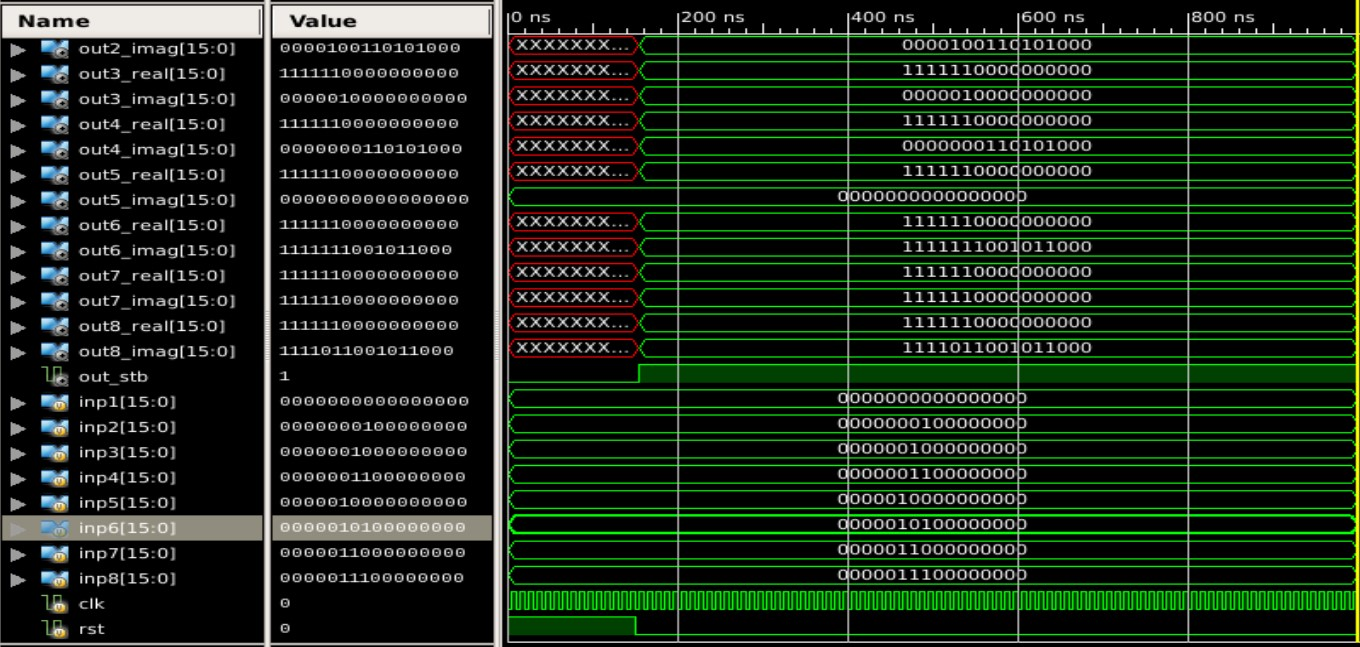
\includegraphics[width=1.0\columnwidth]{simulation_images/figure_1.jpg} 
\end{figure}












\section{Modified Cooley–Tukey algorithm }
\label{modified_Cooley_Tukey_algorithm}

\subsection{Overview}
Cooley–Tukey algorithm for 8 point FFT involves 2 multiplication , hence using 2 multiplicative blocks as seen in the first implementation.In this modified algorithm , the multiplications are pipelined to run one by one , by reusing the same multiplier.

\subsection{Calculation}
The calculations of various intermediate complex numbers is divided into groups and executed group by group.The equation involving different groups are mentioned below.

\subsubsection{Group 1}
$
t_1=D(0) + D(4); \\
m_3=D(0) - D(4); \\
t_2=D(6) + D(2); \\
m_6=j*(D(6)-D(2)); \\
t_3=D(1) + D(5); \\
t_4=D(1) - D(5); \\
t_5=D(3) + D(7); \\
t_6=D(3) - D(7); \\ 
t_8=t_5 + t_3; \\
 m_5=j*(t_5-t_3); \\
t_7=t_1 + t_2; \\
m_2=t_1 - t_2; \\
m_0=t_7 + t_8; \\
m_1=t_7 - t_8; \\
m_4=sin(\pi/4)*(t_4 - t_6);\\
$

\subsubsection{Group 2}
$
m_7=-j* sin(\pi/4)*(t_4 + t_6); \\
s_1=m_3 + m_4;\\
s2=m_3 - m_4; \\
s_3=m_6 + m_7;\\
s4=m_6 - m_7; \\
DO(0)=m_0;\\
DO(4)=m_1; \\ 
DO(1)=s_1 + s_3;\\
DO(7)=s_1 - s_3; \\
DO(2)=m_2 + m_5;\\
DO(6)=m_2 - m_5; \\
DO(5)=s_2 + s_4;\\
DO(3)=s_2 - s_4; \\
$

where D and DO are input and output arrays of the complex data $t_1$,…,$t_8$, $m_1$,…,
$m_7$, $s_1$,…,$s_4$ are the intermediate complex results. As we see the algorithm contains only 2 multiplications to the untrivial coefficient sin($\pi$/4) = 0.7071, and 22 real additions and subtractions. The multiplication to a coefficient j means the negation the imaginary part and swapping real and imaginary parts.


\subsection{Implementation}

The below code implements the \hyperref[modified_Cooley_Tukey_algorithm]{Modified Cooley–Tukey algorithm }. inp1,...inp8 are the 16 bit signed floating point inputs of Q format and out1-real , out1-imag, ...,out8-real,out8-imag are the real and imaginary outputs in 16 bit Q format of the FFT8 module.clk , rst are the clock , reset inputs respectively , and output-stb is the output strobe , which is enabled once the output is calculated.
multiplier module takes inp1, inp2 16 bit signed floating point inputs of Q format and outputs the product of the inputs to out.The module multiplier is initialized once and reused twice in the main FFT8 block .

\begin{lstlisting}[style={verilog-style}]
`timescale 1ns / 1ps

module multiplier(
    input signed [15:0] inp1,
    input signed [15:0] inp2,
    output signed[15:0] out
    );
	reg signed [31:0] inp12;
	always @ ( * )
		begin
			inp12 = inp1*inp2;
		end
	assign out = inp12 [23:8];
endmodule


module fft8(
	input signed [15:0] inp1,
	input signed [15:0] inp2,
	input signed [15:0] inp3,
	input signed [15:0] inp4,
	input signed [15:0] inp5,
	input signed [15:0] inp6,
	input signed [15:0] inp7,
	input signed [15:0] inp8,
	input clk,
	input rst,
	output signed [15:0] out1_real,
	output signed [15:0] out1_imag,
	output signed [15:0] out2_real,
	output signed [15:0] out2_imag,
	output signed [15:0] out3_real,
	output signed [15:0] out3_imag,
	output signed [15:0] out4_real,
	output signed [15:0] out4_imag,
	output signed [15:0] out5_real,
	output signed [15:0] out5_imag,
	output signed [15:0] out6_real,
	output signed [15:0] out6_imag,
	output signed [15:0] out7_real,
	output signed [15:0] out7_imag,
	output signed [15:0] out8_real,
	output signed [15:0] out8_imag,
	output out_stb
);
	
	localparam signed sin_45 = 16'b00000000_10110101;
	localparam signed sin_315 = 16'b11111111_01001011;
	localparam signed sf = 2.0**-8.0;

	reg signed [31:0] t1_46,t2_46; 
	reg signed [15:0] t1,t2,t3,t4,t5,t6,t7,t8,m0,m1,m2,m3,m4;
	reg signed [15:0] m7_imag,s1,s2,s3_imag,s4_imag,m5_imag,m6_imag;
	reg [15:0] mult_inp1,mult_inp2;
	wire [15:0] mult_out;
	reg [1:0] stage;
	reg output_stb;

	multiplier mult (.inp1(mult_inp1), .inp2(mult_inp2), .out(mult_out));

	initial
		begin
			stage = 2'b00;
			output_stb = 1'b0;
		end

	always @( posedge clk)
		begin
			if (rst == 1'b1)
				begin
					output_stb = 1'b0;
				end
			if (stage == 2'b00 && rst == 1'b0)
				begin
					$display("stage-1");
					t1 = inp1 + inp5;
					t2 = inp7 + inp3;
					t3 = inp2 + inp6;
					t5 = inp4 + inp8;
					m3 = inp1 - inp5;
					m6_imag = inp7 - inp3;
					t4 = inp2 - inp6;
					t6 = inp4 - inp8;
					t8 = t5 + t3;
					t7 = t1 + t2;
					m0 = t7 + t8;
					mult_inp1 = t4 - t6;
					mult_inp2 = sin_45;
					stage = 2'b01;
				end
			else if (stage == 2'b01)
				begin
					$display("stage-2");
					m4 = mult_out;
					m5_imag = t5 - t3;
					m2 = t1 - t2;
					m1 = t7 - t8;
					mult_inp1 = t4 + t6;
					mult_inp2 = sin_315;
					stage = 2'b10;
				end
			else if (stage == 2'b10)
				begin
					m7_imag = mult_out;
					s1 = m3 + m4;
					s2 = m3 - m4;
					s3_imag = m6_imag + m7_imag;
					s4_imag = m6_imag - m7_imag;
					stage = 2'b00;
					output_stb = 1'b1;
				end
		end
	assign out_stb = output_stb;
	assign out1_real = m0;
	assign out1_imag = 16'b0000000000000000;
	assign out2_real = s1;
	assign out2_imag = s3_imag;
	assign out3_real = m2;
	assign out3_imag = m5_imag;
	assign out4_real = s2;
	assign out4_imag = ~s4_imag + 1'b1;
	assign out5_real = m1;
	assign out5_imag = 16'b0000000000000000;
	assign out6_real = s2;
	assign out6_imag = s4_imag;
	assign out7_real = m2;
	assign out7_imag = ~m5_imag + 1'b1;
	assign out8_real = s1;
	assign out8_imag = ~s3_imag + 1'b1;
endmodule

\end{lstlisting}

The above code with Test Bench is available in FFT8\_implementation\_2 directory of the project GIT repository.

\subsection{Analysis}
This algorithm calculates the intermediate values in FFT block serially hence reusing the multipliers. Since multipliers are reused , the input bandwidth reduces by half from previous implementation , since 2 clock cycles are needed to perform 2 multiplications one by one.
since both the multiplications happen in serial , total 1 multiplier is only used in this block to evaluate , hence reducing speed . Number of LUTs used is increased since multiplexers are implemented in LUT now to reuse the multiplier by changing inputs in alternate clock cycles . The simulation of this algorithm is shown in \textbf{Figure 2}.

\begin{figure}[h!]
  \caption{Simulation In ISIM}
  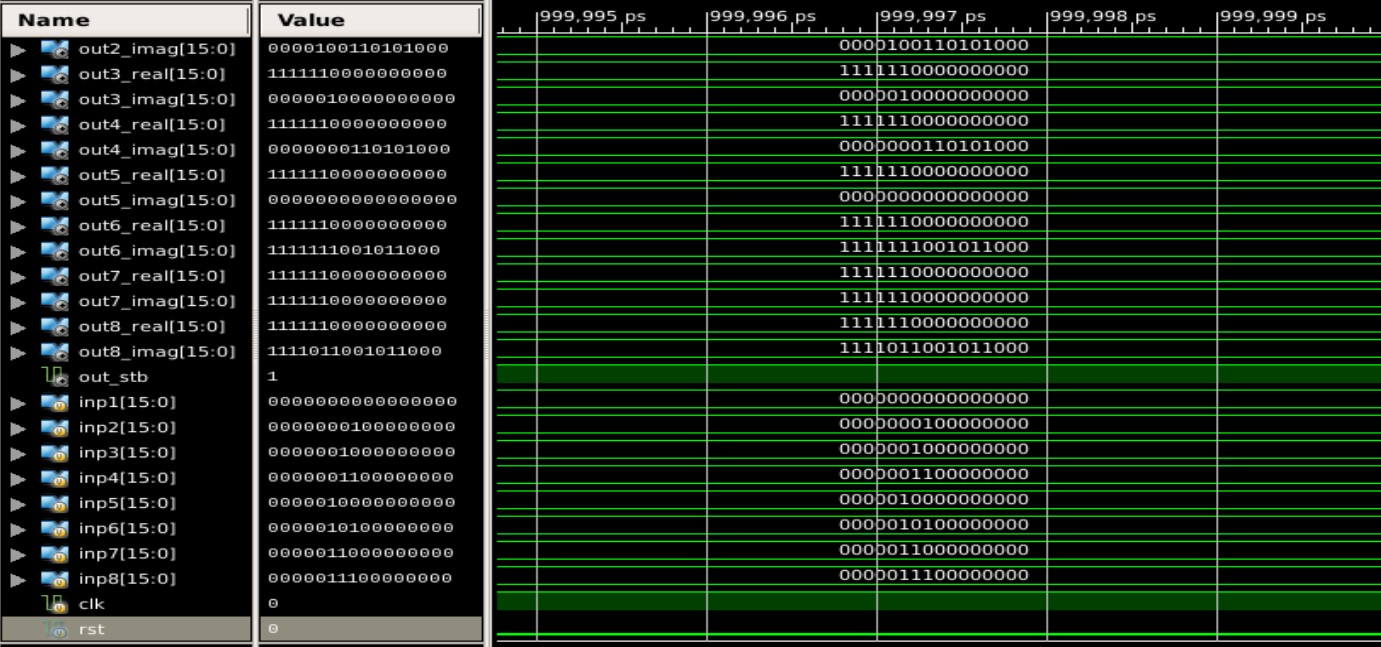
\includegraphics[width=1.0\columnwidth]{simulation_images/figure_2.jpg} 
\end{figure}


\section{Modified Cooley–Tukey algorithm using LUT based Multiplier}

\subsection{Overview}
Cooley–Tukey algorithm for 8 point FFT involves 2 multiplication , hence using 2 multiplicative blocks as seen in the first implementation.In this modified algorithm , the multiplications are pipelined to run one by one , and using a LUT based 16 bit signed multiplier , reducing number of dedicated multiplier blocks , but increasing number of LUTs used.

\subsection{Implementation}

The below code implements the Modified Cooley–Tukey algorithm using LUT based multiplier. inp1,...inp8 are the 16 bit signed floating point inputs of Q format and out1-real , out1-imag, ...,out8-real,out8-imag are the real and imaginary outputs in 16 bit Q format of the FFT8 module.clk , rst are the clock , reset inputs respectively , and output-stb is the output strobe , which is enabled once the output is calculated.
multiplier module takes inp1, inp2 16 bit signed floating point inputs of Q format and outputs the product of the inputs to out.The module multiplier is initialized once and reused twice in the main FFT8 block .
The multiplier module takes input of 2 Q format number , and using Shift-Add algorithm , it multiplies the numbers and outputs every 16 clock cycles.

\begin{lstlisting}[style={verilog-style}]

`timescale 1ns / 1ps

module multiplier(
    input signed [15:0] inp1,
    input signed [15:0] inp2,
	 input rst,
	 input clk,
    output signed [15:0] out,
	 output out_stb
);
   localparam sf = 2.0**-8.0;
	reg [29:0] inp12;
	reg [14:0] input_1;
	reg [14:0] input_2;
	reg output_stb;	
	reg out_sign;
	integer counter;
	assign out_stb = output_stb;
	initial 
		begin
			output_stb = 1'b0;
			inp12 = 32'b0;
			counter = 0;
		end

always @ ( posedge clk )
begin
if (rst == 1'b1)
	begin
	output_stb = 1'b0;
	inp12 = 30'b0;	
	counter = 0;
	end
else if (output_stb == 1'b0 && counter < 15)
	begin
	if (counter == 0)
	begin 
	out_sign = (inp1[15] && ~ inp2 [15]) + (inp2[15] && ~ inp1 [15]);
	input_1 = inp1[15]==1'b0 ? inp1[14:0] : ~inp1[14:0]+1'b1; 
	input_2 = inp2[15]==1'b0 ? inp2[14:0] : ~inp2[14:0]+1'b1; 
	end
	if(input_1[counter]==1'b1)
	begin
	inp12[29:14] = inp12[29:14] + input_2[14:0];
	end
	inp12 = inp12 >> 1;
	counter = counter + 1;
	end
else if (counter >= 15)
	begin
		output_stb = 1'b1;					
	end 
end
assign out = {out_sign,inp12[22:7]};
endmodule



module fft8(
	input signed [15:0] inp1,
	input signed [15:0] inp2,
	input signed [15:0] inp3,
	input signed [15:0] inp4,
	input signed [15:0] inp5,
	input signed [15:0] inp6,
	input signed [15:0] inp7,
	input signed [15:0] inp8,
	input clk,
	input rst,
	output signed [15:0] out1_real,
	output signed [15:0] out1_imag,
	output signed [15:0] out2_real,
	output signed [15:0] out2_imag,
	output signed [15:0] out3_real,
	output signed [15:0] out3_imag,
	output signed [15:0] out4_real,
	output signed [15:0] out4_imag,
	output signed [15:0] out5_real,
	output signed [15:0] out5_imag,
	output signed [15:0] out6_real,
	output signed [15:0] out6_imag,
	output signed [15:0] out7_real,
	output signed [15:0] out7_imag,
	output signed [15:0] out8_real,
	output signed [15:0] out8_imag,
	output out_stb
);
	
	localparam signed sin_45 = 16'b00000000_10110101;
	localparam signed sin_315 = 16'b11111111_01001011;
	localparam signed sf = 2.0**-8.0;

	reg signed [31:0] t1_46,t2_46; 
	reg signed [15:0] t1,t2,t3,t4,t5,t6,t7,t8,m0,m1,m2,m3,m4;
	ref signed [15:0] m5_imag,m6_imag,m7_imag,s1,s2,s3_imag,s4_imag;
	reg [15:0] mult_inp1,mult_inp2;
	wire [15:0] mult_out;
	reg [1:0] stage;
	reg output_stb,mult_rst;
	wire mult_stb;

	multiplier mult (
		.inp1(mult_inp1), 
		.inp2(mult_inp2), 
		.rst(mult_rst), 
		.out(mult_out), 
		.clk(clk),
		.out_stb(mult_stb)
	);

	initial
		begin
			stage = 2'b00;
			output_stb = 1'b0;
			mult_rst = 1'b1;
		end

	always @( posedge clk)
		begin
			if (rst == 1'b1)
				begin
					output_stb = 1'b0;
					mult_rst = 1'b1;
				end
			if (stage == 2'b00 && rst == 1'b0 && output_stb == 1'b0)
				begin
					t1 = inp1 + inp5;
					t2 = inp7 + inp3;
					t3 = inp2 + inp6;
					t5 = inp4 + inp8;
					m3 = inp1 - inp5;
					m6_imag = inp7 - inp3;
					t4 = inp2 - inp6;
					t6 = inp4 - inp8;
					t8 = t5 + t3;
					t7 = t1 + t2;
					m0 = t7 + t8;
					mult_inp1 = t4 - t6;
					mult_inp2 = sin_45;
					stage = 2'b01;
					mult_rst = 1'b0;
				end
			else if (stage == 2'b01 && mult_stb == 1'b1)
				begin
					m4 = mult_out;
					mult_rst = 1'b1;
					stage = 2'b10;
				end
			else if (stage == 2'b10)
				begin
					m5_imag = t5 - t3;
					m2 = t1 - t2;
					m1 = t7 - t8;
					mult_inp1 = t4 + t6;
					mult_inp2 = sin_315;
					mult_rst = 1'b0;
					stage = 2'b11;
				end
			else if (stage == 2'b11 && mult_stb == 1'b1)
				begin
					m7_imag = mult_out;
					s1 = m3 + m4;
					s2 = m3 - m4;
					s3_imag = m6_imag + m7_imag;
					s4_imag = m6_imag - m7_imag;
					mult_rst = 1'b1;
					stage = 2'b00;
					output_stb = 1'b1;
				end
		end
	assign out_stb = output_stb;
	assign out1_real = m0;
	assign out1_imag = 16'b0000000000000000;
	assign out2_real = s1;
	assign out2_imag = s3_imag;
	assign out3_real = m2;
	assign out3_imag = m5_imag;
	assign out4_real = s2;
	assign out4_imag = ~s4_imag + 1'b1;
	assign out5_real = m1;
	assign out5_imag = 16'b0000000000000000;
	assign out6_real = s2;
	assign out6_imag = s4_imag;
	assign out7_real = m2;
	assign out7_imag = ~m5_imag + 1'b1;
	assign out8_real = s1;
	assign out8_imag = ~s3_imag + 1'b1;
endmodule

\end{lstlisting}

The above code with Test Bench is available in FFT8\_implementation\_3 directory of the project GIT repository.


\subsection{Analysis}
This algorithm calculates the intermediate values in FFT block serially hence reusing the multipliers. Since multipliers are reused , the input bandwidth reduces by half from implementation where 2 multiplier blocks are used. Since the multiplier is LUT based , the usage of LUTs increase , but it reduces the amount number of DSP48A1s which are very scarce in FPGAs.

\begin{figure}[h!]
  \caption{Simulation In ISIM}
  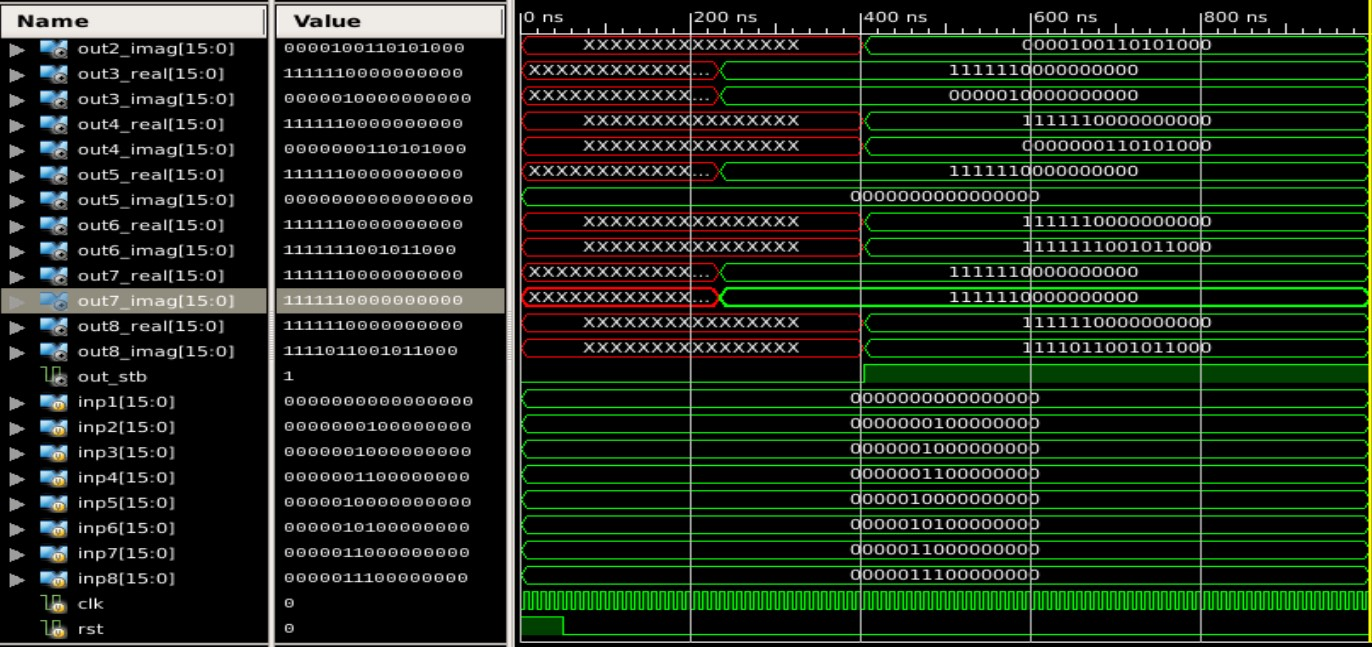
\includegraphics[width=1.0\columnwidth]{simulation_images/figure_3.jpg} 
\end{figure}





\section{Validation Script}
A python Validation script is written to validate the FFT Verilog Blocks. The python script below uses Numpy library to generate 100 random floating point test inputs and using ISIM command line options simulates all the inputs and validates them with the standard FFT function present in the numpy library of python.


\definecolor{codegreen}{rgb}{0,0.6,0}
\definecolor{codegray}{rgb}{0.5,0.5,0.5}
\definecolor{codepurple}{rgb}{0.58,0,0.82}
\definecolor{backcolour}{rgb}{0.95,0.95,0.92}
 
\lstdefinestyle{python-style}{
    backgroundcolor=\color{backcolour},   
    commentstyle=\color{codegreen},
    keywordstyle=\color{magenta},
    numberstyle=\tiny\color{codegray},
    stringstyle=\color{codepurple},
    basicstyle=\footnotesize,
    breakatwhitespace=false,         
    breaklines=true,                 
    captionpos=b,                    
    keepspaces=true,                 
    numbers=left,                    
    numbersep=5pt,                  
    showspaces=false,                
    showstringspaces=false,
    showtabs=false,                  
    tabsize=2,
    language=Python
}

\begin{lstlisting}[style={python-style}]

import numpy as np
from bitstring import Bits
import os
implement=raw_input("design to test(allowed values 1,2,3)")
working_directory=r"/FFT8_implementation_"+str(implement)

print("Generating 100 Random Inputs ... ")
cmds = ""
for i in range(100):
  input_array=np.random.uniform(low=-8.0, high=8.0, size=(8,))
  binary_array=[]
  for inp in input_array:
    binary_array.append(Bits(int=int(inp*2**8), length=16).bin)
  cmd="""
   isim force add {/fft8_tb/inp1} %s -radix bin 
   isim force add {/fft8_tb/inp2} %s -radix bin 
   isim force add {/fft8_tb/inp3} %s -radix bin 
   isim force add {/fft8_tb/inp4} %s -radix bin 
   isim force add {/fft8_tb/inp5} %s -radix bin 
   isim force add {/fft8_tb/inp6} %s -radix bin 
   isim force add {/fft8_tb/inp7} %s -radix bin 
   isim force add {/fft8_tb/inp8} %s -radix bin 
   isim force add {/fft8_tb/clk} 1 -radix bin -value 0 -radix
   bin -time 2500 ps -repeat 5 ns -cancel 1 us
   isim force add {/fft8_tb/rst} 1 -radix bin -cancel 20 ns 
   isim force add {/fft8_tb/rst} 0 -radix bin -time 20 ps
   -cancel 1 us 
   run
   dump
  """%tuple(binary_array)
  cmds=cmds+cmd

os.chdir(working_directory)
f=open("inp.test","w")
f.write(cmds)
f.close()
print("Simulating all the inputs using ISIM...")
cmd='"'+working_directory+r'/fft8_tb_isim_beh.exe" < inp.test > out.test'
os.system(cmd)
f=open("out.test","r")
values=[]
inp={}
out={}
for line in f.readlines():
 print line
 if "Signal:" in line:
  out[line.strip().split("{")[1].split("}")[0].split("[")[0].strip()]=line.strip().split(":")[-1].strip()
 if "Variable:" in line:
  inp[line.strip().split("{")[1].split("}")[0].split("[")[0].strip()]=line.strip().split(":")[-1].strip()
 if "{rst}" in line.strip():
  values.append([inp,out])
  inp={}
  out={}

f.close()

print("Verifying FFT output with the actual values...")
correct=0
count=0
for val in values:
  count=count+1
  inp = np.asarray([Bits(bin=val[0]['inp'+str(i)]).int/(2.0**8) for i in range(1,9)])
  out1 = np.array([Bits(bin=val[1]['out'+str(i)+"_real"]).int/(2.0**8) for i in range(1,9)])
  out2 = np.array([Bits(bin=val[1]['out'+str(i)+"_imag"]).int/(2.0**8) for i in range(1,9)])
  out=out1 + 1j*out2
  if np.allclose(out,np.fft.fft(inp),1e-2):
   correct=correct+1

print(str(correct)+r"/"+str(count)+" Correct ...")




\end{lstlisting}

\subsection{Requirements}
\begin{itemize}
  \item >=Python 2.7
  \item bitstring library
  \item ISIM simulator
\end{itemize}

\subsection{Sample Usage}
\begin{figure}[h!]
  \caption{Python 2.7}
  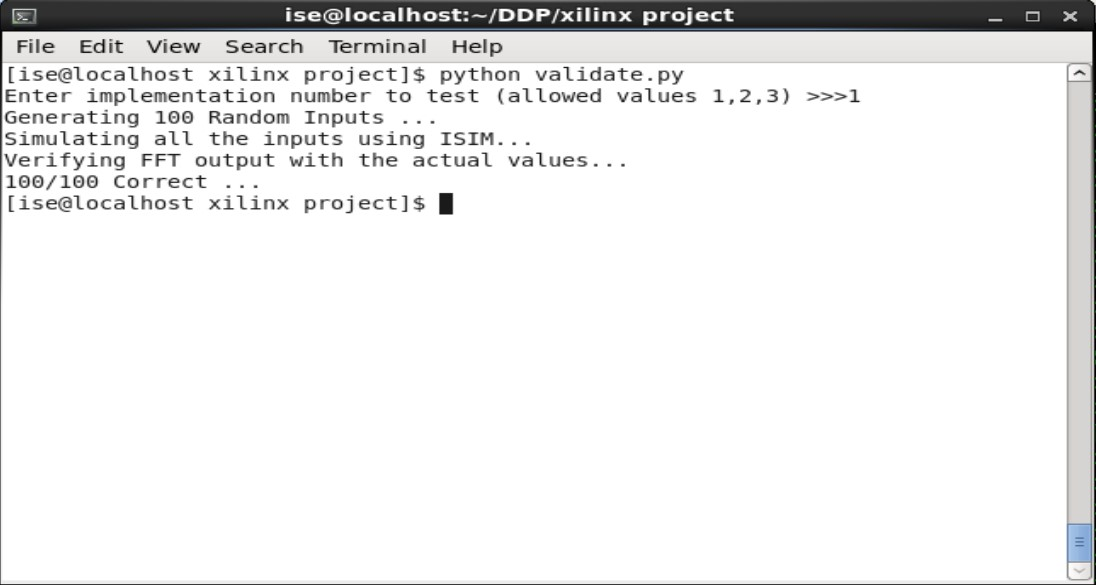
\includegraphics[width=1.0\columnwidth]{simulation_images/figure_4.jpg} 
\end{figure}

Clone the GIT repository from the URL given in the project link section, and run validate.py script to validate the designs.
The validate.py file is present in the root folder of the GIT repository.Sample usage of the script is shown in figure 4.

\section{Project URL}
Project GIT repository: \href {https://github.com/Mohankumariitm/Dual-Degree-Project}{https://github.com/Mohankumariitm/Dual-Degree-Project}
Use Git or checkout with SVN using the web URL.

\section{Design Summary}
Below is the resource utilization summary of the above implementations.


\begin{center}
\begin{tabular}{ |c|c|c|c| } 
 \hline
Logic Utilization & Implementation 1 & Implementation 2 & Implementation 3 \\ [0.8ex] 
 \hline
Number of Slice Registers & 47 & 317 & 357 \\
 \hline
Number of Slice LUTs & 337 & 374 & 456 \\
 \hline
Number of fully used LUT-FF pairs & 47 & 138 & 188 \\
 \hline
Number of BUFG/BUFGCTRLs & 1 & 1 & 1 \\
 \hline
Number of DSP48A1s & 2 & 1 & 0 \\
 \hline
\end{tabular}
\end{center}


\section{To Do (in upcoming months)}:
\href {https://www.embedded.com/design/connectivity/4403178/Doing-Hartley-Smartly}https://www.embedded.com/design/connectivity/4403178/Doing-Hartley-Smartly

\begin{itemize}
  \item Implement FFT using Doing-Hartley-Smartly Method, and Analyze the resource usage
  \item Implement Variations in Doing-Hartley-Smartly Method by reusing resources to reduce the LUTs.
\end{itemize}



\end{document}




